\chapter{Ideas probadas: lo que funcionó y lo que no}
\label{cap:extensiones}

Este capítulo reúne seis extensiones que se plantearon como preguntas sobre el fútbol, más que como mejoras del pronóstico. Cuatro dieron resultados negativos limpios, con pruebas calibradas para poder detectar un efecto si existía. Una, la de eventos raros, es una herramienta de Monte Carlo y funcionó.

\section{¿Hay intransitividad? (R4)}

Si existieran estilos que se anulan (el equipo A le gana a B, B a C y C a A con más frecuencia de la que explican las fuerzas), aparecerían como ciclos en el grafo de resultados de una temporada. La descomposición de Hodge~\cite{jiang2011} separa un flujo sobre las aristas en una parte gradiente (explicable por un potencial, que es una fuerza), una parte rotacional local (ciclos de tres) y una parte armónica (ciclos globales).

\begin{proposicion}[Sin componente armónica] \dem
En una liga todos contra todos el grafo es completo, el complejo de cliques no tiene ciclos no triviales y la componente armónica es nula: toda la intransitividad es local.
\end{proposicion}

\begin{proof}
El complejo de cliques del grafo completo de $N$ vértices es el $2$-esqueleto del símplice de dimensión $N-1$, que es contráctil; su primera homología es trivial y, por la teoría de Hodge combinatoria, el espacio armónico de dimensión uno, isomorfo a $H^1$, es nulo.
\end{proof}

La prueba compara la proporción cíclica observada (la fracción de la energía del flujo en la parte rotacional) con su distribución bajo un modelo de fuerzas puras, simulada por bootstrap paramétrico desde un modelo ajustado a cada temporada. En 108 temporadas, la proporción observada es 0,596 frente a 0,590 del nulo, y la combinación de Fisher de los valores $p$ da $p=0{,}81$. Chile es la liga más ``cíclica'' (0,72), pero dentro de su nulo.

\begin{nota}{Un nulo mal elegido da el resultado al revés}
La primera versión usaba como nulo las predicciones un paso adelante del filtro, y daba que la realidad era \emph{más} transitiva que el nulo. La pista estaba en el signo: esas predicciones están contraídas hacia la media, porque son estimaciones con incertidumbre, y las temporadas simuladas con ellas tienen fuerzas más parejas y por lo tanto más ciclos. El nulo correcto simula desde fuerzas ajustadas a la temporada completa.
\end{nota}

\section{¿Hay estilos latentes? (R5)}

Un término bilineal $u_i^\top v_j$ sobre el predictor del filtro permitiría que el ataque de $i$ interactúe con la defensa de $j$ más allá de las fuerzas, como en los modelos de factores latentes de redes~\cite{hoff2005}.

\begin{proposicion}[Umbral nuclear] \dem
El MAP de $(U,V)$ con prior $\N(0,s^2)$ en cada entrada resuelve $\min_\Gamma\ \ell(\Gamma)+\|\Gamma\|_*/s^2$, y su solución es $\Gamma=0$ si y solo si $\|\nabla\ell(0)\|_2\le1/s^2$.
\end{proposicion}

\begin{proof}
Por la caracterización variacional de la norma nuclear~\cite{recht2010},
\[
\|\Gamma\|_*=\min_{UV^\top=\Gamma}\tfrac12\big(\|U\|_F^2+\|V\|_F^2\big),
\]
así que minimizar sobre $(U,V)$ equivale a minimizar sobre $\Gamma$ con penalización nuclear. El problema es convexo y $\Gamma=0$ es óptimo si y solo si $0\in\nabla\ell(0)+\partial\|\cdot\|_*(0)/s^2$; el subdiferencial de la norma nuclear en cero es la bola unitaria de la norma espectral.
\end{proof}

La pregunta ``¿hay estilos?'' se convierte en una prueba espectral: comparar el mayor valor singular de la matriz de residuos atacante $\times$ defensor (doblemente centrada, para eliminar errores aditivos de fuerza) con su distribución bajo el modelo sin interacción. El mayor valor singular observado (8,55) queda bajo el percentil 95 del nulo (9,66) en todas las ligas. Con $s=0{,}2$ el MAP es exactamente nulo, como predice la proposición, y con $s\ge0{,}5$ sobreajusta: empeora la predicción entre 38 y 68 milinats por partido. Además, el MAP conjunto con una escala jerárquica es degenerado (el embudo de Neal~\cite{neal2003}: la densidad diverge cuando $s\to0$ con $U=V=0$), así que la escala se fija o se integra con NUTS.

\section{Dentro del partido (R8, R9)}
\label{sec:envivo}

Con la línea de tiempo de goles y tarjetas de 21.730 partidos se ajusta un proceso de conteo con intensidad log-lineal por tramos de 15 minutos y estados (marcador, tarjetas rojas). La verosimilitud es la de un GLM de Poisson sobre 572 mil segmentos (``piecewise exponential''), y las probabilidades en vivo resuelven las ecuaciones de Kolmogorov hacia adelante $\dot p=pQ(t)$ con $Q$ constante por tramos, mediante exponenciales de matriz.

\begin{figure}[h]
\centering
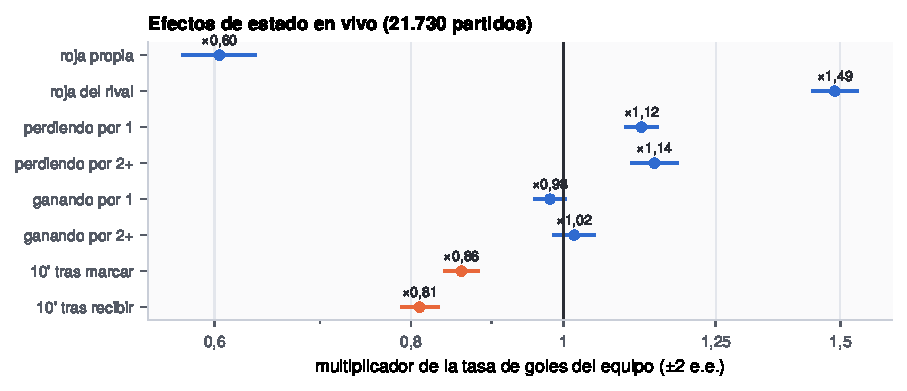
\includegraphics[width=\textwidth]{envivo}
\caption{Multiplicadores de la tasa de goles de un equipo según el estado del partido, con intervalos de dos errores estándar. En naranja, los diez minutos siguientes a un gol.}
\label{fig:envivo}
\end{figure}

Los efectos de estado son grandes y esperables (figura~\ref{fig:envivo}): una roja propia multiplica la tasa de goles por 0,60 y una del rival por 1,49; ir perdiendo por uno, por 1,12. Los tiempos de descuento equivalen a unos 2,3 minutos en el primer tiempo y 5,5 en el segundo. El resultado interesante es el del contagio (R9). Un proceso de Hawkes~\cite{hawkes1971} aditivo, en el que cada gol aumenta temporalmente la tasa de goles, estima una excitación nula. Con el modelo multiplicativo el efecto es significativo pero al revés: en los diez minutos siguientes a un gol, el que anotó marca $\times0{,}86$ y el que recibió $\times0{,}81$ (razón de verosimilitudes 363). Los goles no se contagian: se inhiben, con un período refractario de celebración, saque y reacomodo táctico.

\section{¿Llega tarde el filtro? (R10)}

Un paseo aleatorio gaussiano se mueve de a poco, y un equipo que cambia de golpe (un nuevo entrenador, una lesión clave) tardaría en reflejarse. Para medirlo se corre una detección bayesiana de cambios en línea~\cite{adams2007} sobre los residuos de diferencia de gol de cada equipo, con prior Normal–Gamma (predictiva $t$ de Student).

\begin{observacion} \dem
Con tasa de riesgo constante $H$, $P(r_t=0\mid x_{1:t})=H$ siempre: un cambio en $t$ no es identificable con el dato de $t$. La detección se hace con retraso, con $P(r_{t+d}\le d\mid x_{1:t+d})$.
\end{observacion}

Si el filtro llegara tarde, después de cada cambio detectado los residuos seguirían sesgados en la dirección del cambio. Tras 132 detecciones, el residuo medio de los 10 partidos siguientes es $0{,}025\pm0{,}046$: el filtro se pone al día solo.

\section{Probabilidades de una en un millón (R12)}

El muestreo por importancia de la sección~\ref{sec:raros} se validó contra fuerza bruta: ``el City termina 10.º o peor'' da $2{,}41\cdot10^{-4}\pm5$\,\% frente a $2{,}48\cdot10^{-4}\pm8$\,\% con 600.000 temporadas directas, con quince veces menos simulación por igual error. Con semillas consistentes entre sí: el City desciende con probabilidad $\approx2\cdot10^{-7}$ (una en cinco millones), el PSG $\approx7\cdot10^{-7}$, el Gladbach, último, sale campeón con $\approx8\cdot10^{-7}$ y el Bournemouth, último, con $\approx1{,}2\cdot10^{-4}$. Bajo $10^{-8}$ las semillas discrepan y solo se reporta el orden de magnitud. En Chile y Brasil, con la liga avanzada, los mismos eventos son imposibles por la cota entera.

\section{El mercado de pases (R14, R15)}

\parrafo{Como señal de pretemporada.} Para cada club y temporada, el balance de traspasos normalizado, $x_i=(V^\text{llega}_i-V^\text{sale}_i)/\operatorname{mediana}_j(V^\text{llega}_j+V^\text{sale}_j)$, debería anticipar cuánto mejora un equipo más allá de lo que el filtro espera. Dentro de muestra el coeficiente es $\gamma=0{,}04\pm0{,}01$, pero fuera de muestra (2016-2025) la correlación es $-0{,}04$ y el pronóstico de pretemporada empeora levemente. Para los ascendidos el coeficiente es mayor (0,11), pero aplicarlo solo a ellos es neutro. La regresión a la media del filtro ya captura lo que el mercado anticipa.

\parrafo{Como aristas entre ligas.} Un traspaso definitivo de la liga $A$ a la $B$ se modeló como una comparación por pares sobre las fuerzas netas de la red. Con 8.377 traspasos, la jerarquía que implican no se correlaciona con la de los partidos (Spearman $-0{,}02$): la Serie B y LaLiga 2 ``atraen'' más que la Premier y la Ligue 1 ``exporta''. El mercado mide dinero, no nivel deportivo. La validación cruzada en partidos de copa elige $\beta=0$ y empeora de forma monótona al subirlo. Forzarlos habría bajado la resistencia Inglaterra–Chile de 0,134 a 0,050: una precisión falsa.

\begin{conclusion}
\textsf{\bfseries\color{cdblue}Lectura de conjunto.} Lo que funciona es más estructura en el modelo de goles (separar crear de convertir), propagar la incertidumbre honestamente y un mejor Monte Carlo. Lo que no funciona son las ideas que suponen más estructura en el juego que la que hay en los datos (estilos, ciclos, rachas) y la información de mercado que el filtro ya contiene. La lección de método vino de un error de datos: revisar la consistencia de los datos antes de concluir un negativo cambió la conclusión sobre los tiros al arco.
\end{conclusion}
